\documentclass[onecolumn, 11pt,openany]{memoir}

% packages
\usepackage{blindtext, color}
\usepackage[usenames,dvipsnames,svgnames,table,xcdraw]{xcolor}
\usepackage{graphicx}  
\usepackage{import}  
\usepackage[english]{babel}
\usepackage[outline]{contour} 
\usepackage{ctable}
\newcolumntype{d}[1]{D{.}{.}{#1}}
\usepackage[utf8]{inputenc}
\usepackage[compact]{titlesec}
\usepackage{pdfpages}
\usepackage{float}
\usepackage{lmodern}
% \usepackage{microtype}
\definecolor{lightgray}{gray}{0.9}
\usepackage{multicol}
\usepackage{authblk}

% font and lay-out
%current font: BT Charter. Find other fonts at http://www.tug.dk/FontCatalogue/
\usepackage[bitstream-charter]{mathdesign}
\usepackage[T1]{fontenc}

%caption layout
\usepackage[format=plain]{caption}
\DeclareCaptionLabelSeparator{bar}{ | }
\captionsetup[figure]{labelfont={bf},name={Figure},labelsep=bar,font=footnotesize}
\captionsetup[table]{labelfont={bf},name={Table},labelsep=bar,font=footnotesize}

%symbols
\usepackage{textcomp}
\usepackage{gensymb}
\usepackage[euler]{textgreek}

% paragraph indent & spacing
\setlength\parskip{\baselineskip}
\setlength\parindent{0pt} % use 0 pt for no indent

% page sizes and margins
\usepackage[a4paper, margin=1in]{geometry}

% dummy text; just for testing
\usepackage{lipsum}

% hyphenation
% list all hy-phe-na-ted words as they should be hyphenated
% to repress hyphenation place word (or two) in an mbox operator; e.g.:  \mbox{P. infestans} 

\hyphenation{hy-phe-na-te}

\label{START}
\begin{document}
\thispagestyle{empty}                   
\frontmatter

\title{Increasing readability of your preprint by typesetting}
\author[1,2]{Author 1}
\author[1]{Author 2}
\author[3]{Author 3}
\begin{scriptsize}
\affil[1]{University 1}
\affil[2]{University 2}
\affil[3]{University 3}
\end{scriptsize}
\date{\vspace{-5ex}} % this is workaround to remove date and move main text up. For printing date remove vspace operator
\maketitle

\subsection{Correspondence}
Please address correspondence to firstname.lastname@univ.edu

\pagenumbering{arabic}
\pagestyle{plain}

\section{Abstract}
A very simple \LaTeX{} template for preprint formatting. LaTeX does have a pretty steep learning curve, but once you get the hang of it it'll be amazing.  Feel free to edit according to your preferences. I give zero promise for correct typesetting or the absence of errors, but it should not give much troubles.

The attached .tex file (see GitHub) contains the minimum (maybe not the bare minimum) amount of packages, so in case you want to have more freedom add more packages to your needs. Doing so gives possibility to include page-spanning tables, for example, or have parts of the document printed in landscape format.

The code is available via: https://github.com/hooge104/preprint\_template\_latex

\begin{multicols}{2}
\section{Introduction}
\lipsum[2-5]

\section{Results}
\subsection{Experiment 1}
\lipsum[6-8]

%figure referencing as following. Remove \textbf operator to print links not bold
These data show us that we successfully silenced our favourite gene \textbf{Figure ~\ref{fig1}}. All primers used in this study are listed in \textbf{Table ~\ref{tabS1_primers}}.

\begin{figure*}[t]
\centering
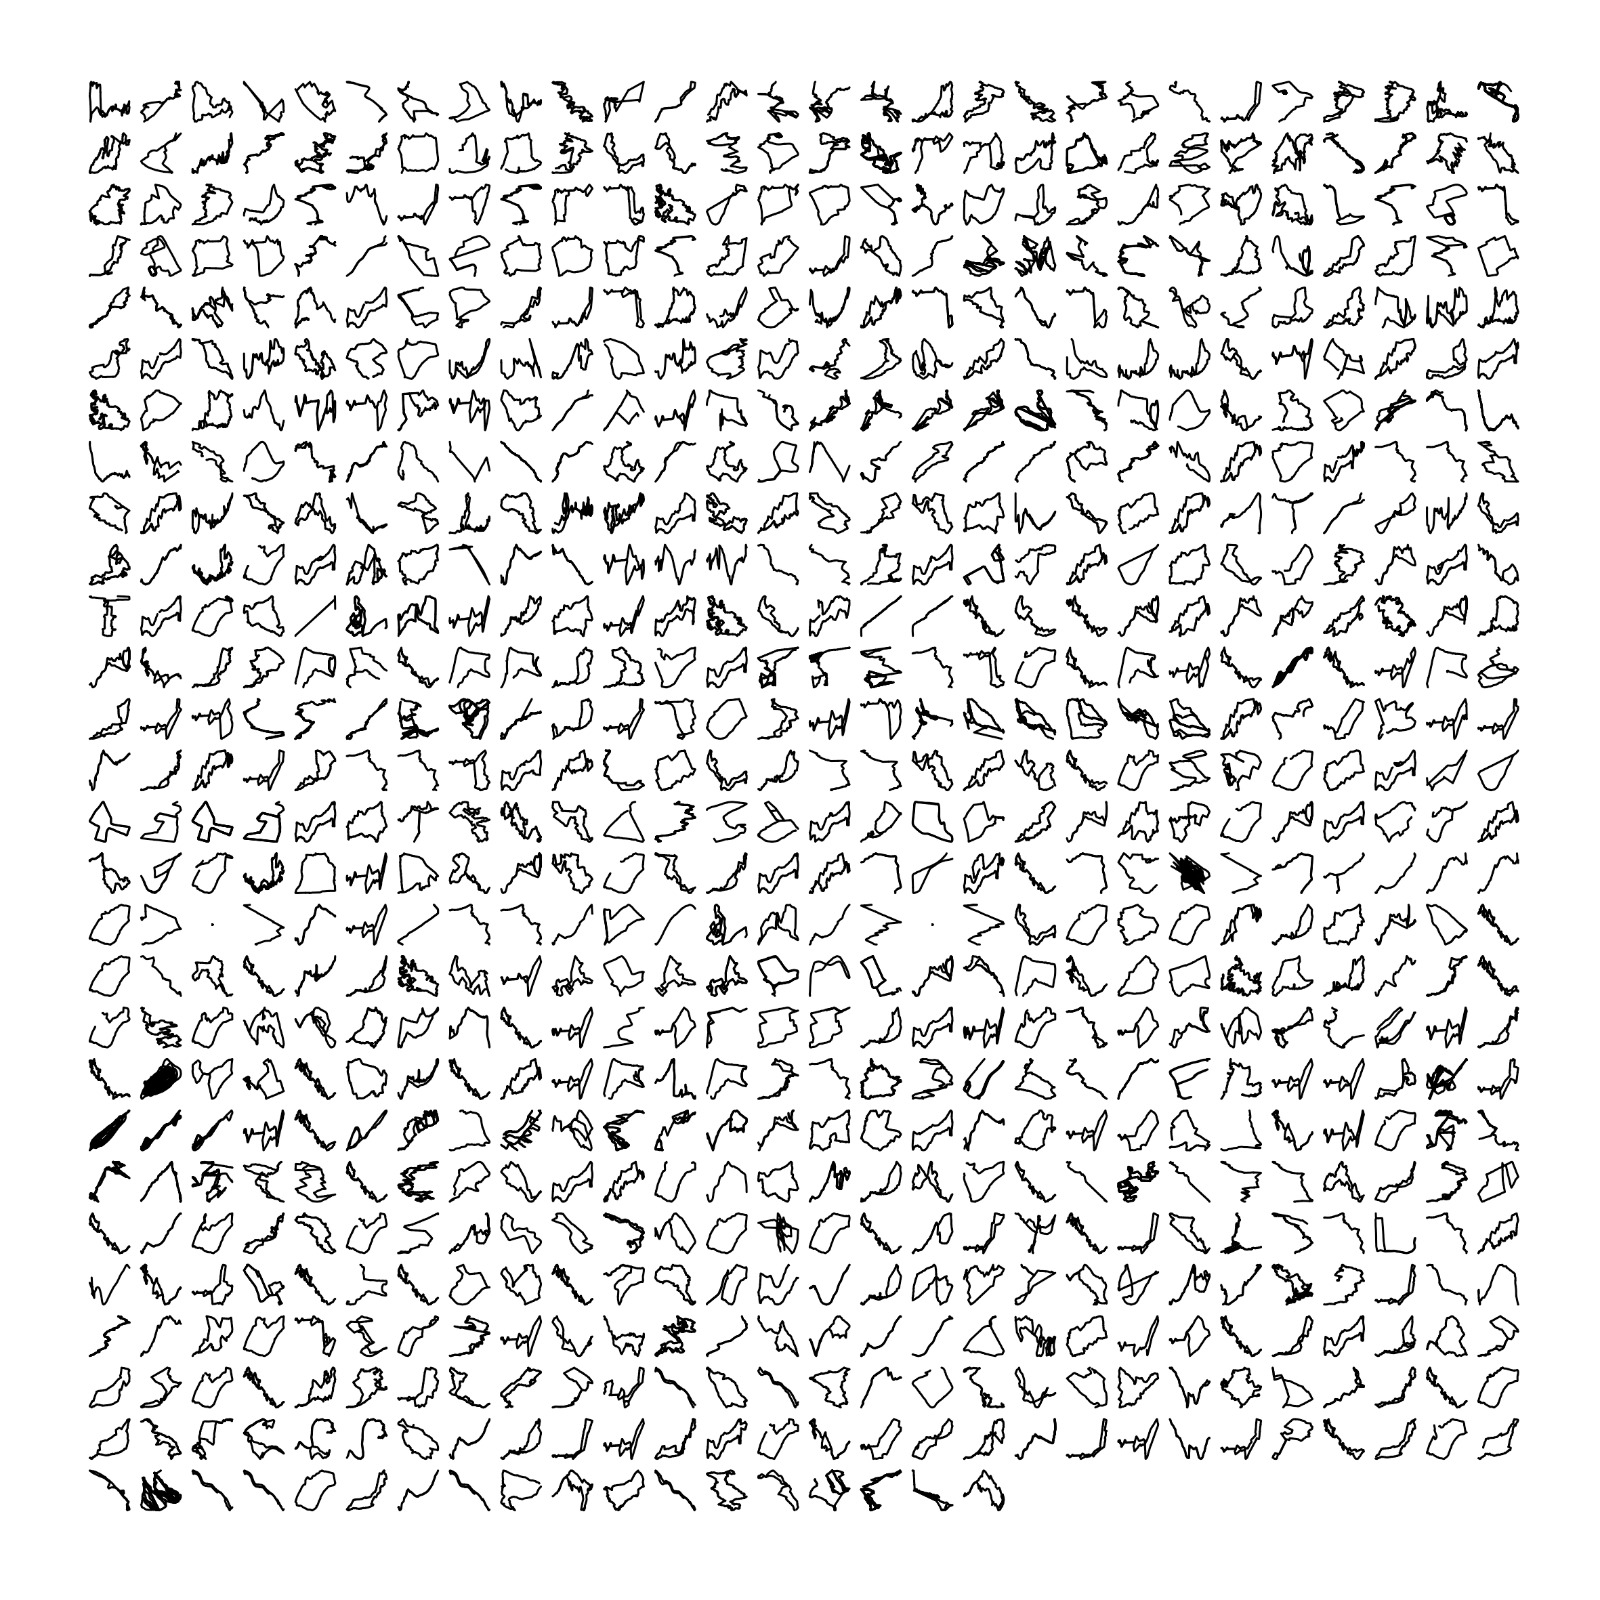
\includegraphics[width=1\textwidth]{Figures/Fig1}
\caption{\textbf{Caption title.} \textbf{a)} Subfigure description. \textbf{b)} Subfigure description.}
\label{fig1}
\end{figure*}

\subsection{Experiment 2}
\lipsum[9]

\subsection{Experiment 3}
\lipsum[10]

\begin{figure*}[hb]
\centering
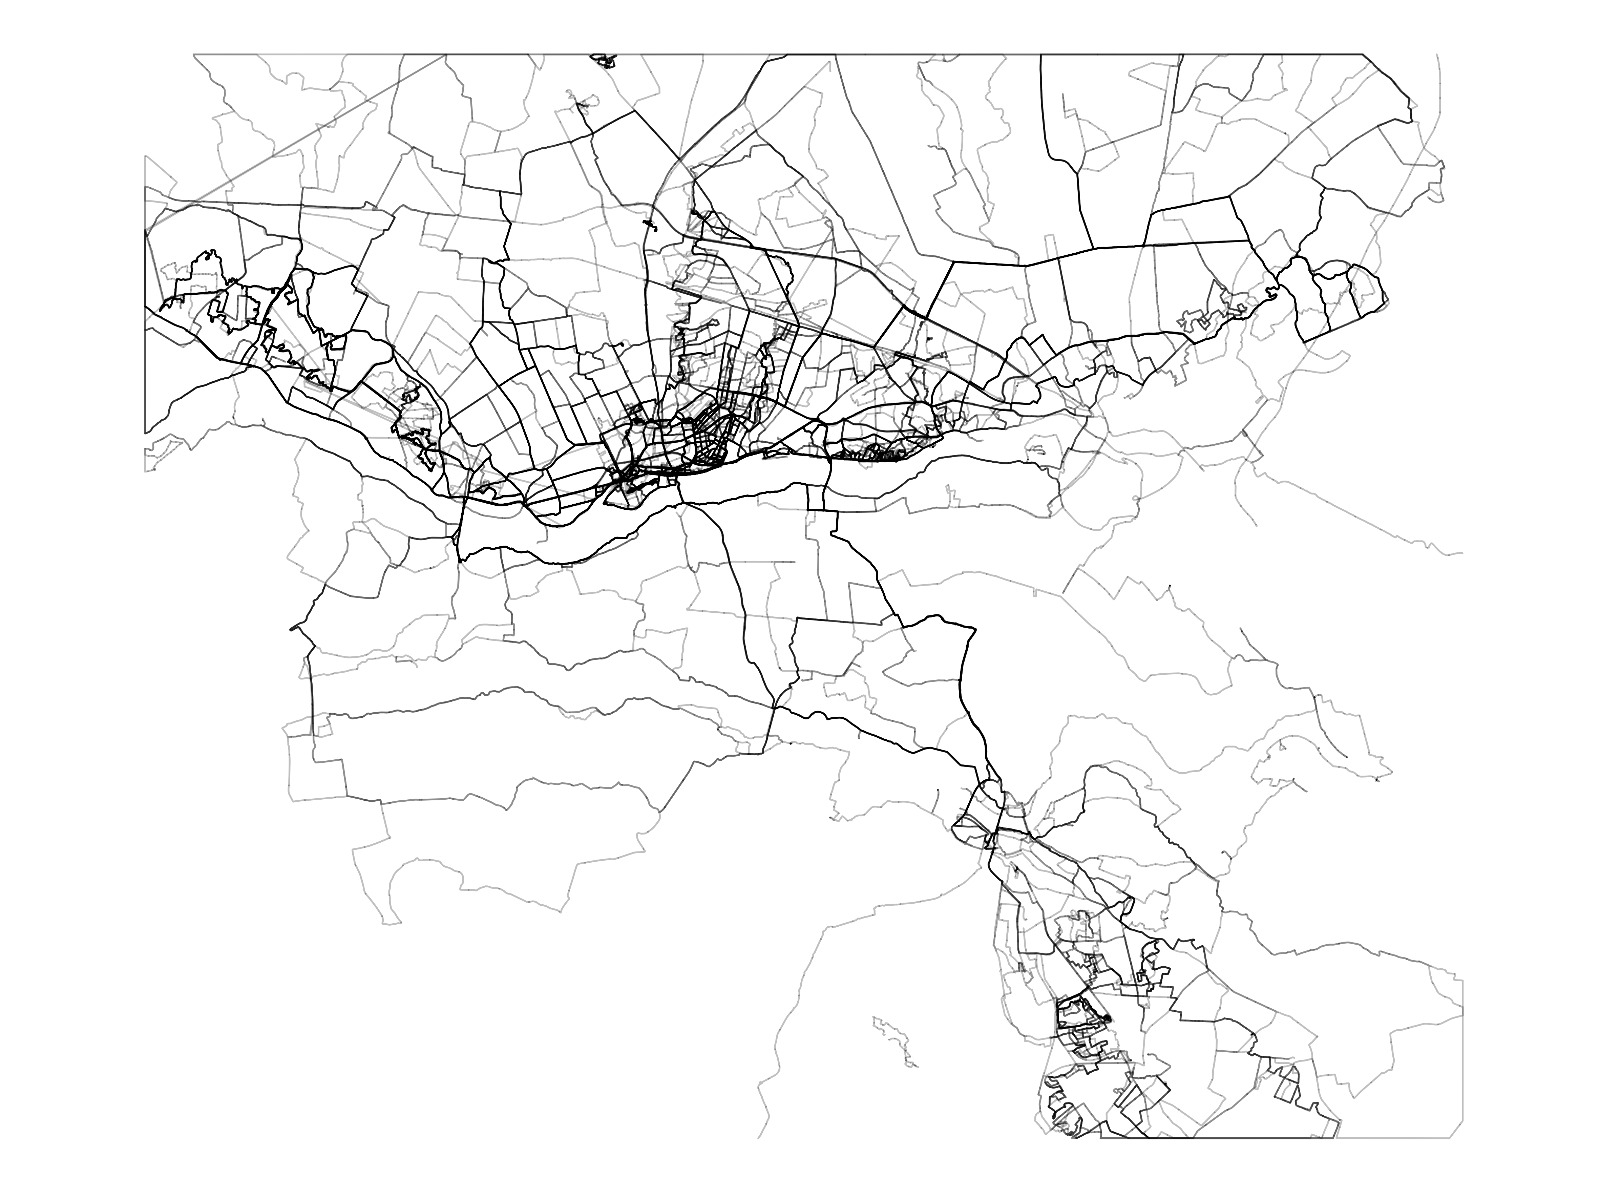
\includegraphics[width=0.9\textwidth]{Figures/Fig2}
\caption{\textbf{Caption title.} \textbf{a)} Subfigure description. \textbf{b)} Subfigure description.}
\label{fig2}
\end{figure*}

\subsection{Experiment 4}
\lipsum[1]

\subsubsection{Sub experiment a}
\lipsum[1]

\subsubsection{Sub experiment b}
\lipsum[1]

\subsubsection{Sub experiment c}
\lipsum[1]

\section{Discussion}
\lipsum[1-6]

\section{Acknowledgements}
We are grateful to our colleagues who generously shared their constructs and experiences. This work was supported by xxx with financial aid from the xxx in the framework of the xxx programme (project \# 1234).

\begin{footnotesize}
\section{Materials and methods}

\subsection{Culturing conditions}
\lipsum[1]

\subsection{Experimental procedures}
\lipsum[1]

\subsection{Constructs}
\lipsum[1]

\section{Data availability}
All data is public available under xxx.

\end{footnotesize}

\section{References}
\setlength\parindent{-0.5 em}
\setlength{\parskip}{0 em}
\setlength{\leftskip}{0.5 em}

\begin{sloppy}
\begin{footnotesize}
Ah-Fong, A. M., C. A. Bormann-Chung and H. S. Judelson (2008). Optimization of transgene-mediated silencing in \textit{Phytophthora infestans} and its association with small-interfering RNAs, \textit{Fungal Genet Biol} \textbf{45}: 1197-1205. doi: 10.1016/j.fgb.2008.05.009

Ah-Fong, A. M. and H. S. Judelson (2011). Vectors for fluorescent protein tagging in \textit{Phytophthora}: tools for functional genomics and cell biology, \textit{Fungal Biol} \textbf{115}: 882-890. doi: 10.1016/j.funbio.2011.07.001

Brinkman, E. K., T. Chen, M. Amendola and B. van Steensel (2014). Easy quantitative assessment of genome editing by sequence trace decomposition, \textit{Nucleic Acids Res} \textbf{42}: e168. doi: 10.1093/nar/gku936

Caten, C. E. and J. L. Jinks (1968). Spontaneous Variability of Single Isolates of \textit{Phytophthora infestans}. Cultural Variation, \textit{Can J Botany} \textbf{46}: 329-348. doi: 10.1139/b68-055

Chen, F., S. M. Pruett-Miller, Y. Huang, M. Gjoka, K. Duda, J. Taunton, . . . G. D. Davis (2011). High-frequency genome editing using ssDNA oligonucleotides with zinc-finger nucleases, \textit{Nat Methods} \textbf{8}: 753-755. doi: 10.1038/nmeth.1653

Cho, S. W., J. Lee, D. Carroll, J. S. Kim and J. Lee (2013). Heritable gene knockout in \textit{Caenorhabditis elegans} by direct injection of Cas9-sgRNA ribonucleoproteins, \textit{Genetics} \textbf{195}: 1177-1180. doi: 10.1534/genetics.113.155853

Doench, J. G., E. Hartenian, D. B. Graham, Z. Tothova, M. Hegde, I. Smith, . . . D. E. Root (2014). Rational design of highly active sgRNAs for CRISPR-Cas9-mediated gene inactivation, \textit{Nat Biotechnol} \textbf{32}: 1262-1267. doi: 10.1038/nbt.3026

Fang, Y. and B. M. Tyler (2016). Efficient disruption and replacement of an effector gene in the oomycete \textit{Phytophthora sojae} using CRISPR/Cas9, \textit{Mol Plant Pathol} \textbf{17}: 127-139. doi: 10.1111/mpp.12318

Gamboa-Melendez, H., A. I. Huerta and H. S. Judelson (2013). bZIP transcription factors in the oomycete \textit{Phytophthora infestans} with novel DNA-binding domains are involved in defense against oxidative stress, \textit{Eukaryot Cell} \textbf{12}: 1403-1412. doi: 10.1128/EC.00141-13

Govers, F. and M. Gijzen (2006). \textit{Phytophthora }genomics: the plant destroyers' genome decoded, \textit{Mol Plant Microbe Interact} \textbf{19}: 1295-1301. doi: 10.1094/MPMI-19-1295

Grahl, N., E. G. Demers, A. W. Crocker and D. A. Hogan (2017). Use of RNA-Protein Complexes for Genome Editing in Non-albicans \textit{Candida} Species, \textit{mSphere} \textbf{2}. doi: 10.1128/mSphere.00218-17

Gumtow, R., D. Wu, J. Uchida and M. Tian (2017). A \textit{Phytophthora palmivora} extracellular cystatin-like protease inhibitor targets papain to contribute to virulence on papaya, \textit{Mol Plant Microbe Interact}. doi: 10.1094/MPMI-06-17-0131-FI

Judelson, H. S. (1997). The genetics and biology of \textit{Phytophthora infestans}: modern approaches to a historical challenge, \textit{Fungal Genet Biol} \textbf{22}: 65-76. doi: 10.1006/fgbi.1997.1006

Kamoun, S., O. Furzer, J. D. Jones, H. S. Judelson, G. S. Ali, R. J. Dalio, . . . F. Govers (2015). The Top 10 oomycete pathogens in molecular plant pathology, \textit{Mol Plant Pathol} \textbf{16}: 413-434. doi: 10.1111/mpp.12190

Kay, J., H. J. G. Meijer, A. ten Have and J. A. van Kan (2011). The aspartic proteinase family of three \textit{Phytophthora }species, \textit{BMC Genomics} \textbf{12}: 254. doi: 10.1186/1471-2164-12-254

Kearse, M., R. Moir, A. Wilson, S. Stones-Havas, M. Cheung, S. Sturrock, . . . A. Drummond (2012). Geneious Basic: an integrated and extendable desktop software platform for the organization and analysis of sequence data, \textit{Bioinformatics} \textbf{28}: 1647-1649. doi: 10.1093/bioinformatics/bts199

Kim, S., D. Kim, S. W. Cho, J. Kim and J. S. Kim (2014). Highly efficient RNA-guided genome editing in human cells via delivery of purified Cas9 ribonucleoproteins, \textit{Genome Res} \textbf{24}: 1012-1019. doi: 10.1101/gr.171322.113

Kleinstiver, B. P., S. Q. Tsai, M. S. Prew, N. T. Nguyen, M. M. Welch, J. M. Lopez, . . . J. K. Joung (2016). Genome-wide specificities of CRISPR-Cas Cpf1 nucleases in human cells, \textit{Nat Biotechnol} \textbf{34}: 869-874. doi: 10.1038/nbt.3620

Lange, A., R. E. Mills, C. J. Lange, M. Stewart, S. E. Devine and A. H. Corbett (2007). Classical nuclear localization signals: definition, function, and interaction with importin alpha, \textit{J Biol Chem} \textbf{282}: 5101-5105. doi: 10.1074/jbc.R600026200

Le Blanc, C., F. Zhang, J. Mendez, Y. Lozano, K. Chatpar, V. Irish and Y. Jacob (2017). Increased efficiency of targeted mutagenesis by CRISPR/Cas9 in plants using heat stress, \textit{Plant J}. doi: 10.1111/tpj.13782

Ramakrishna, S., A. B. Kwaku Dad, J. Beloor, R. Gopalappa, S. K. Lee and H. Kim (2014). Gene disruption by cell-penetrating peptide-mediated delivery of Cas9 protein and guide RNA, \textit{Genome Res} \textbf{24}: 1020-1027. doi: 10.1101/gr.171264.113

Ran, F. A., L. Cong, W. X. Yan, D. A. Scott, J. S. Gootenberg, A. J. Kriz, . . . F. Zhang (2015). In vivo genome editing using Staphylococcus aureus Cas9, \textit{Nature} \textbf{520}: 186-191. doi: 10.1038/nature14299

Ran, F. A., P. D. Hsu, J. Wright, V. Agarwala, D. A. Scott and F. Zhang (2013). Genome engineering using the CRISPR-Cas9 system, \textit{Nat Protoc} \textbf{8}: 2281-2308. doi: 10.1038/nprot.2013.143

Soares Medeiros, L. C., L. South, D. Peng, J. M. Bustamante, W. Wang, M. Bunkofske, . . . R. L. Tarleton (2017). Rapid, Selection-Free, High-Efficiency Genome Editing in Protozoan Parasites Using CRISPR-Cas9 Ribonucleoproteins, \textit{mBio} \textbf{8}. doi: 10.1128/mBio.01788-17

Stajich, J. E., T. Harris, B. P. Brunk, J. Brestelli, S. Fischer, O. S. Harb, . . . D. S. Roos (2012). FungiDB: an integrated functional genomics database for fungi, \textit{Nucleic Acids Res} \textbf{40}: D675-681. doi: 10.1093/nar/gkr918

Van den Hoogen, D. J., H. J. G. Meijer, M. F. Seidl and F. Govers (2018). The ancient link between G-protein coupled receptors and C-terminal phospholipid kinase domains, \textit{mBio} \textbf{9}. doi: 10.1128/mBio.02119-17

\end{footnotesize}
\end{sloppy}
\end{multicols}

\clearpage

\section{Supplementary files}
\makeatletter 
\setcounter{figure}{0}
\renewcommand{\thetable}{S\arabic{table}}   
\renewcommand{\thefigure}{S\arabic{figure}}
\renewcommand{\figurename}{Supplemental Figure}
\renewcommand{\tablename}{Supplemental Table}

\begin{figure*}[h]
\centering
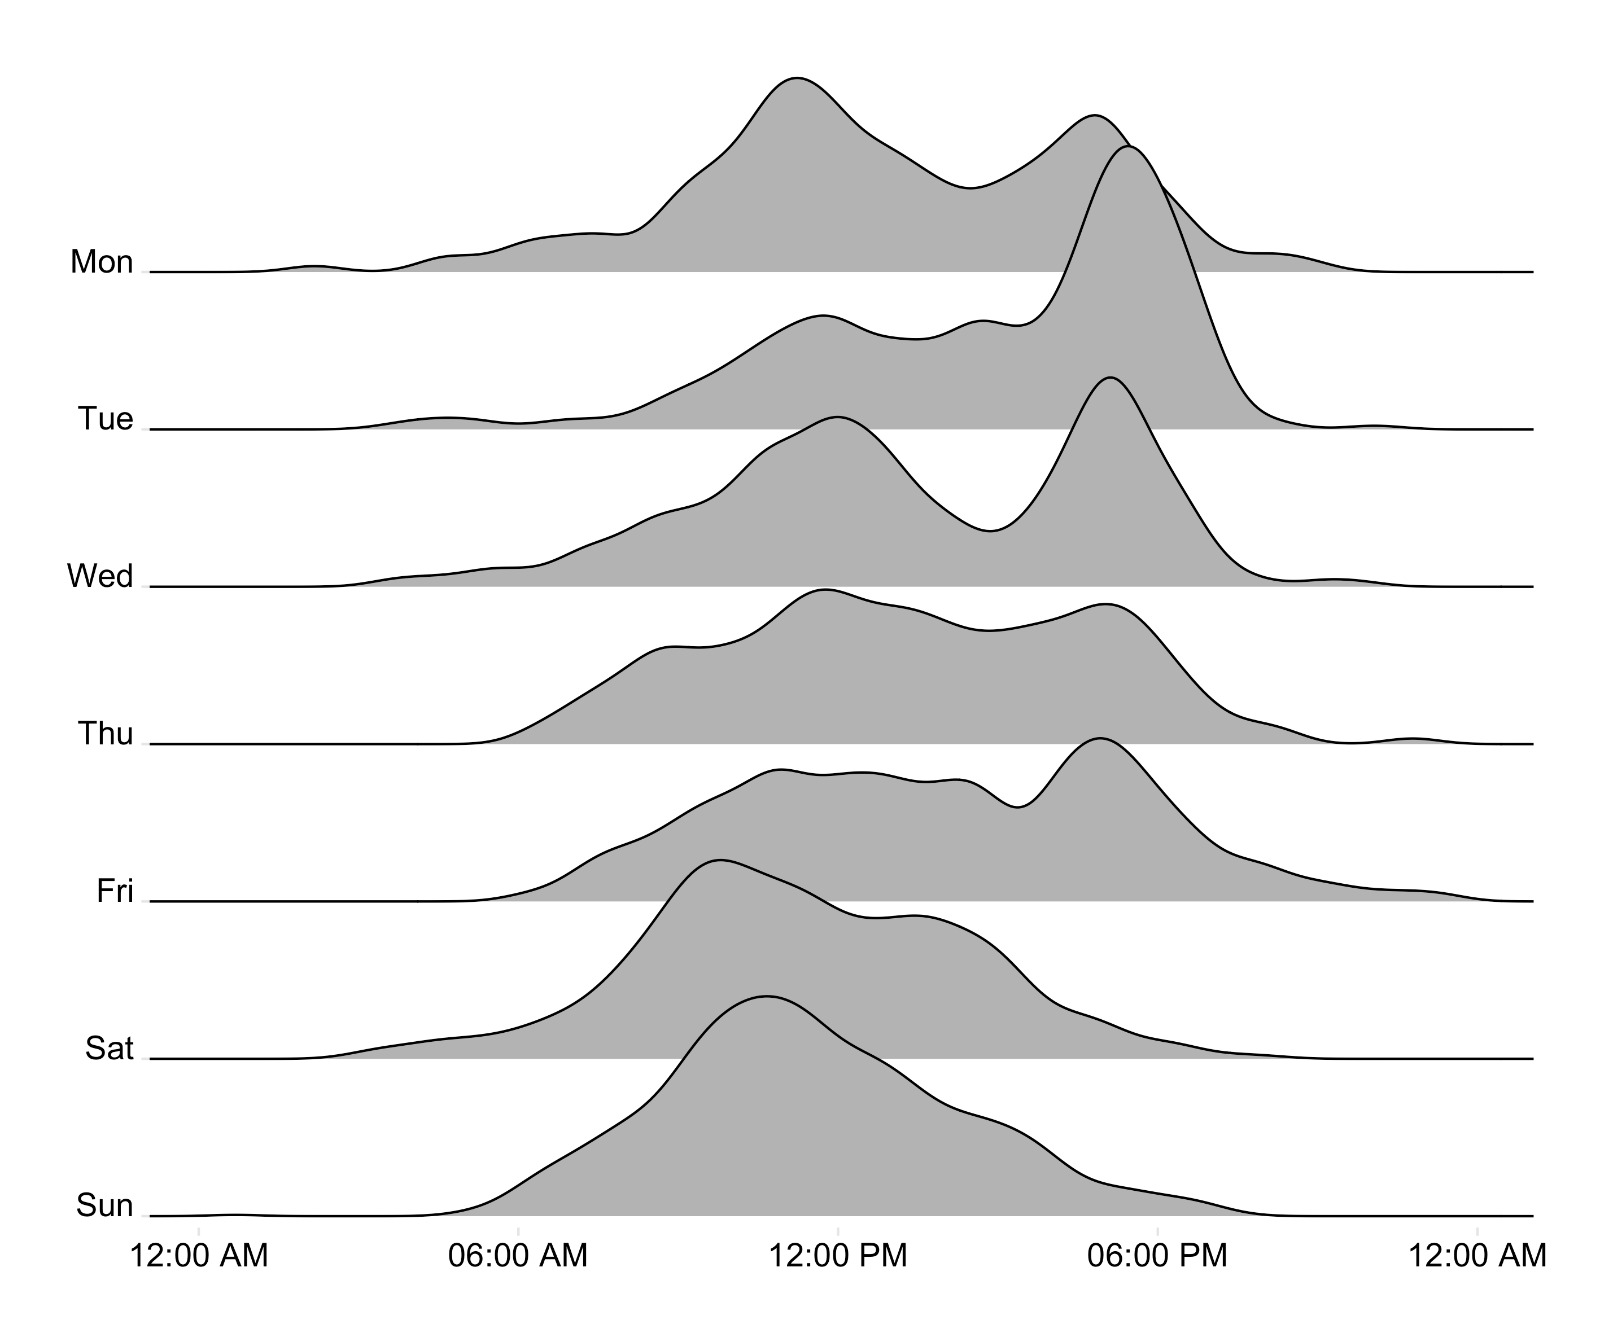
\includegraphics[width=0.7\textwidth]{Figures/FigS1}
\caption{\textbf{Caption title.} \textbf{a)} Subfigure description. \textbf{b)} Subfigure description.}
\label{figS1_detection}
\end{figure*}

\begin{table*}[h]
\rowcolors{0}{}{lightgray}
\centering
\begin{footnotesize}
\caption{\textbf{Primers used in this study}.}
\label{tabS1_primers}
\begin{tabular}{llll}
\hline
\textbf{Name}                     & \textbf{Sequence (5' - 3')}                           & \textbf{Purpose}                                   &  \\ \hline
Primer 1                  & ACTGACGTACTAACACTGACGTACTATGACGTACTA                          & Expression analysis          &  \\
Primer 2                  & ACTGACGTACTACTGACGTACTAGACGTACTAACTA                  & Expression analysis         &  \\
Primer 3         & ACTGACACTGACACTGACGTACTAGTACTAGTACTA    & Cloning                   &  \\
Primer 4     & ACTGACGACTGACACTGACGTACTAGTACTATACTA     & Cloning                          &  \\ \hline
\end{tabular}
\end{footnotesize}
\end{table*}

\end{document}
